\chapter{Implementation and Results}

\section{System Development and Environment Setup}
The basic purpose of this study is to identify the anxiety level of the programmer without disturbing the programming work, creating an artificial environment, or using biological instruments such as EEG caps or heart rate monitors. The reason for this is that for the passive detection of such anxiety, the software was designed as a light-weight background application for C/C++ development, especially for CodeBlocks.

\subsection{Runtime Architecture}

This approach employs a passive runtime architecture implemented directly against the underlying OS' API layer. Instead of implementing an IDE-plugin, which could be subject to version dependency problems, create unnecessary runtime overhead, and possibly give away the monitoring process, this monitor runs asynchronously in the background within the underlying OS.

The system constantly hooks itself into keyboard event stream and active window monitoring. In particular, the architecture is designed for tracking program execution switches between the main IDE (\texttt{codeblocks.exe}), the compiler/debugger (\texttt{gcc.exe} or \texttt{gdb.exe}), and terminal execution windows (\texttt{cmd.exe}). In this way, the decoupled architecture ensures zero-latency influence on the student’s main programming environment. The system logs high-frequency behavioral measures---such as keystroke rates, context switches, and pause times---on a consistent 30-second interval basis. Operating within the underlying OS guarantees the complete ecological validity of the programming test.

\subsection{Rule-Based Anxiety Score Engine}
Before the use of sophisticated machine learning techniques, the Anxiety Score System consisted of an expert-based rule-driven "Anxiety Score Engine." The engine was built using existing Human-Computer Interaction (HCI) rules. For instance, there is a link between erratic typing speeds and high mental workload, while higher backspace frequency typically correlates with frustration and stress.

The engine combined those metrics using a fixed linear equation to produce the \texttt{anxiety\_score} value, which ranges between 0 and 100. Based on that, the system categorized the user’s anxiety state in one of four distinct categories, LOW, MODERATE, HIGH, and CRITICAL. Although the engine was unable to perform dynamic thresholding as compared to trained neural networks or classifiers, it formed the computational metric needed for statistical validation against self-reported measures.

\section{Data Collection Methodology}

\subsection{Study Context and Participant Demographics}
In order to ensure that the model was trained using authentic physiological stress as opposed to a simulated stress response, data collection was conducted directly during active, marked academic examination sessions. The experiment comprised a total of 67 first-year undergraduate computer science students, all of whom were under the age of 25. As the participants were evaluated and graded in real-time, the psychological and physiological stress elicited during the data collection process provides high ecological validity. The exam tasks involved solving programming problems and writing algorithmic logic of varying degrees of complexity under strict time constraints.

\subsection{Automated Data Extraction Workflow}
To ensure the monitoring system operated with zero intrusion and without requiring manual initialization by the students, a customized batch (\texttt{.bat}) script was deployed. This script seamlessly executed the background tracking application via the Windows command prompt, initiating the data collection process silently as soon as the examination began. Figure \ref{fig:bat_cmd} demonstrates the batch script actively capturing keyboard and window interactions through the command line interface in the background.

\begin{figure}[htbp]
    \centering
    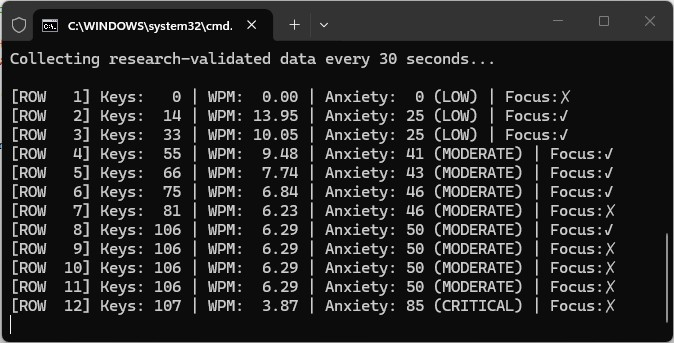
\includegraphics[width=0.8\textwidth]{data_collecting_bat.jpg}
    \caption{Background execution of the data collection monitor via batch (cmd) script.}
    \label{fig:bat_cmd}
\end{figure}

The captured raw behavioral metrics were instantaneously serialized and appended into a Comma-Separated Values (CSV) dataset. This localized logging ensured no network overhead or latency was added to the students' workstations during the critical exam period. Figure \ref{fig:csv_sample} provides a snapshot of the raw dataset generated by the script, highlighting high-frequency variables such as total keystrokes, active window context, latency, and pause durations.

\begin{figure}[htbp]
    \centering
    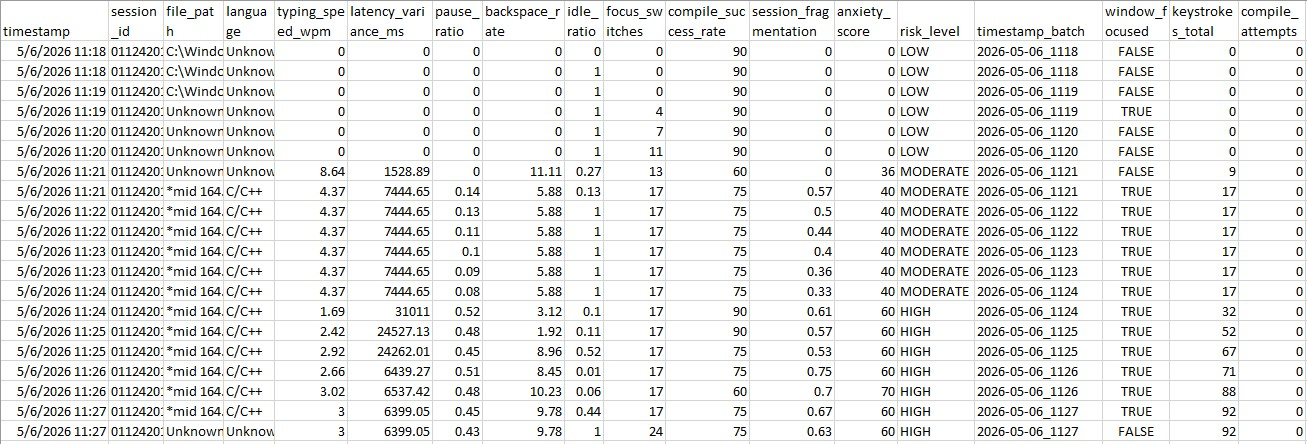
\includegraphics[width=0.95\textwidth]{dataset_csv_sample.jpg}
    \caption{Sample of the raw behavioral dataset logged directly into CSV format.}
    \label{fig:csv_sample}
\end{figure}

\subsection{Data Cleaning and Preprocessing Pipeline}
As mentioned above, the raw behavioral logs collected through the Windows API contained noise intrinsic to any unconstrained human-computer interaction dataset. Thus, a rigorous data cleaning and preprocessing pipeline was implemented prior to the machine learning analysis.

\begin{enumerate}
    \item \textbf{Warm-up Filtering}: The first time-series entries where \texttt{keystrokes\_total} was zero were discarded. This is to avoid the early test-reading phase of the session (when the student is simply reading the problem description) from artificially dragging their average typing speed to false lows.
    \item \textbf{Outlier Capping}: Extreme behavioral anomalies were mathematically capped. For example, if a student took several minutes to ask an invigilator a question, the value of \texttt{latency\_variance\_ms} would jump to astronomical levels. To ensure such mechanical outliers do not distort the mathematical variance calculations, \texttt{latency\_variance\_ms} was capped at a strict threshold of 30,000 milliseconds.
    \item \textbf{Data Merging and Aggregation}: The individual CSV log files generated for each of the 67 students across the four separate examination sessions were computationally merged. This massive data consolidation produced a unified, time-series dataset comprising exactly 11,138 behavioral observations, segmented into consistent 30-second intervals.
\end{enumerate}

\subsection{Exploratory Data Analysis (EDA) and Label Distribution}
However, in supervised machine learning, the effectiveness of the algorithm relies heavily on the quality of its labels. In order to provide the "Ground Truth" for EDA, it was necessary for students to fill out the post-exam survey in the period of 5 to 15 minutes following their test, making sure that the psychological state was still vividly remembered.

Students self-reported the level of perceived stress on a Likert scale of 1 to 5, with 1 meaning low stress, and 5 meaning high stress. Thus, the generated dataset featured natural class imbalance, with the great predominance of stressed students (those at levels 4 and 5). Naturally, this represents the reality of how psychological state during a computer science examination looks like.

\begin{figure}[htbp]
    \centering
    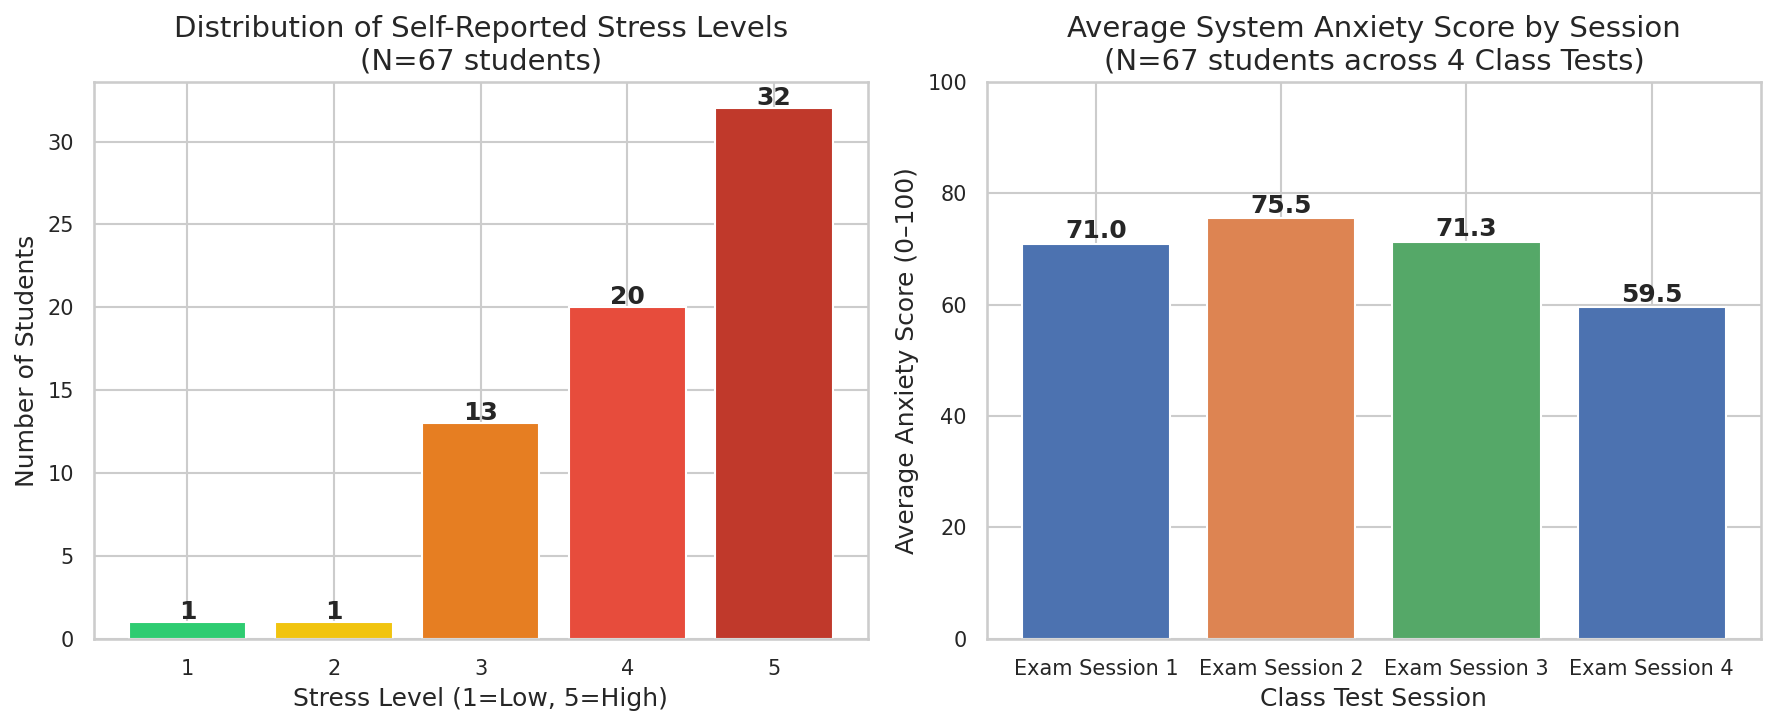
\includegraphics[width=0.9\textwidth]{stress_distribution_by_session.png}
    \caption{Distribution of Self-Reported Stress Levels and Average System Anxiety Score by Session.}
    \label{fig:stress_distribution}
\end{figure}

\section{Validation Against Self-Reported Stress}
Before implementation of any machine learning techniques, it became mathematically necessary to verify the presence of any psychological signal within the raw behavioral data. The validation of the computational \texttt{anxiety\_score}, computed using the rule engine, was achieved by comparing it against the students' self-reported Ground Truth stress values.

By aggregating the 11,138 rows into average profiles for the 67 students, rigorous statistical correlation tests were conducted:

\begin{itemize}
    \item \textbf{Pearson Correlation (Linear Relationship)}: $r = 0.521$ ($p < 0.0001$)
    \item \textbf{Spearman Correlation (Monotonic Relationship)}: $\rho = 0.310$ ($p = 0.0107$)
\end{itemize}

In terms of data mining in psychology, the p-value should be 0.05 to reject the null hypothesis. Both correlation values are statistically significant ($p \ll 0.05$). It absolutely confirms that there is a correlation between the passively recording device and real human anxiety. Every time when the student felt anxious, there was a mathematical change in his interaction with the keyboard.

\begin{figure}[htbp]
    \centering
    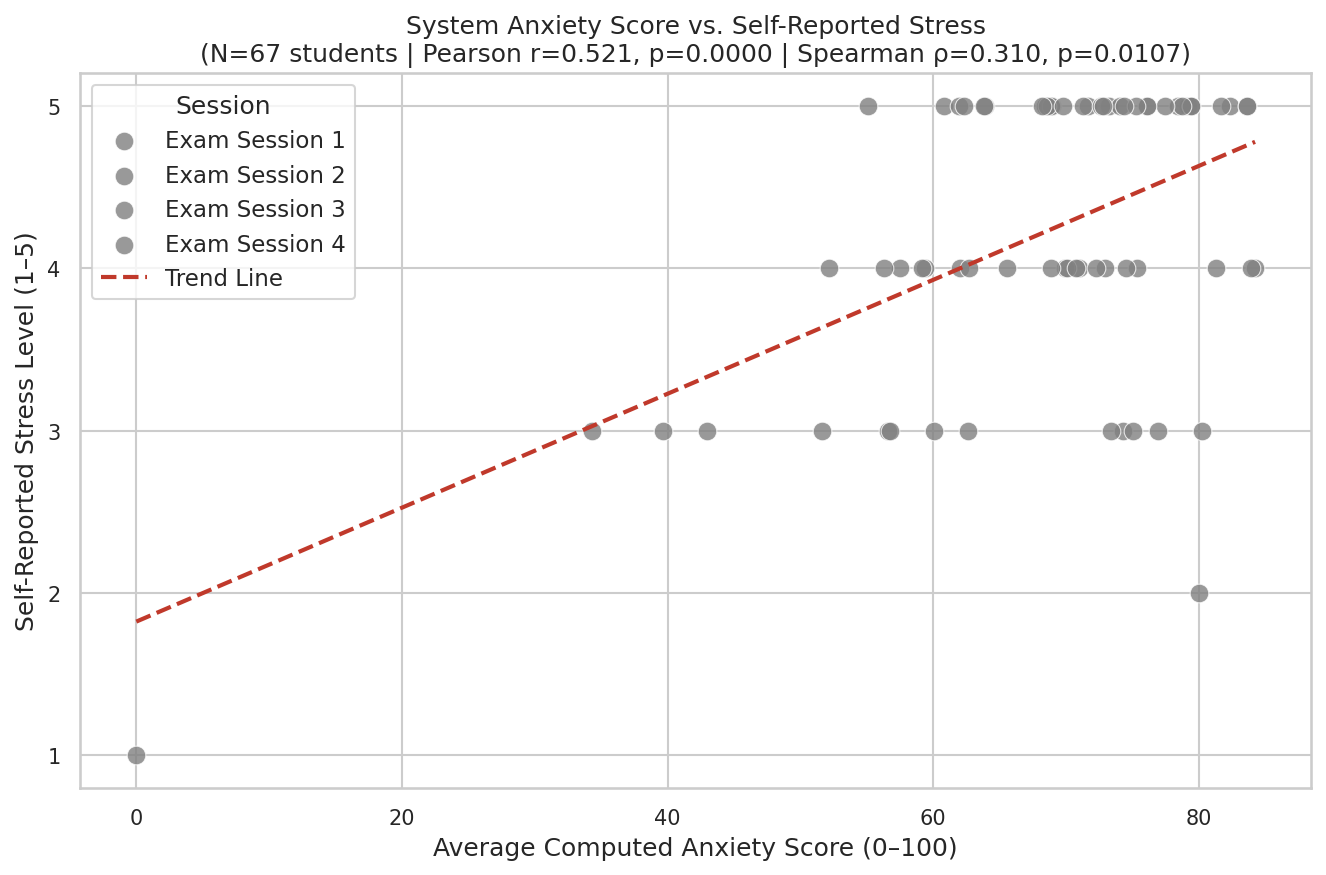
\includegraphics[width=\textwidth]{anxiety_vs_stress_scatter.png}
    \caption{System Anxiety Score vs. Self-Reported Stress Scatter Plot.}
    \label{fig:anxiety_scatter}
\end{figure}

To further understand the interactions between different behavioral vectors, a correlation heatmap was generated. It revealed expected multicollinearity (e.g., idle ratio positively correlating with pause ratio) while highlighting which raw metrics had the strongest individual pull on the final anxiety score.

\clearpage


\begin{figure}[htbp]
    \centering
    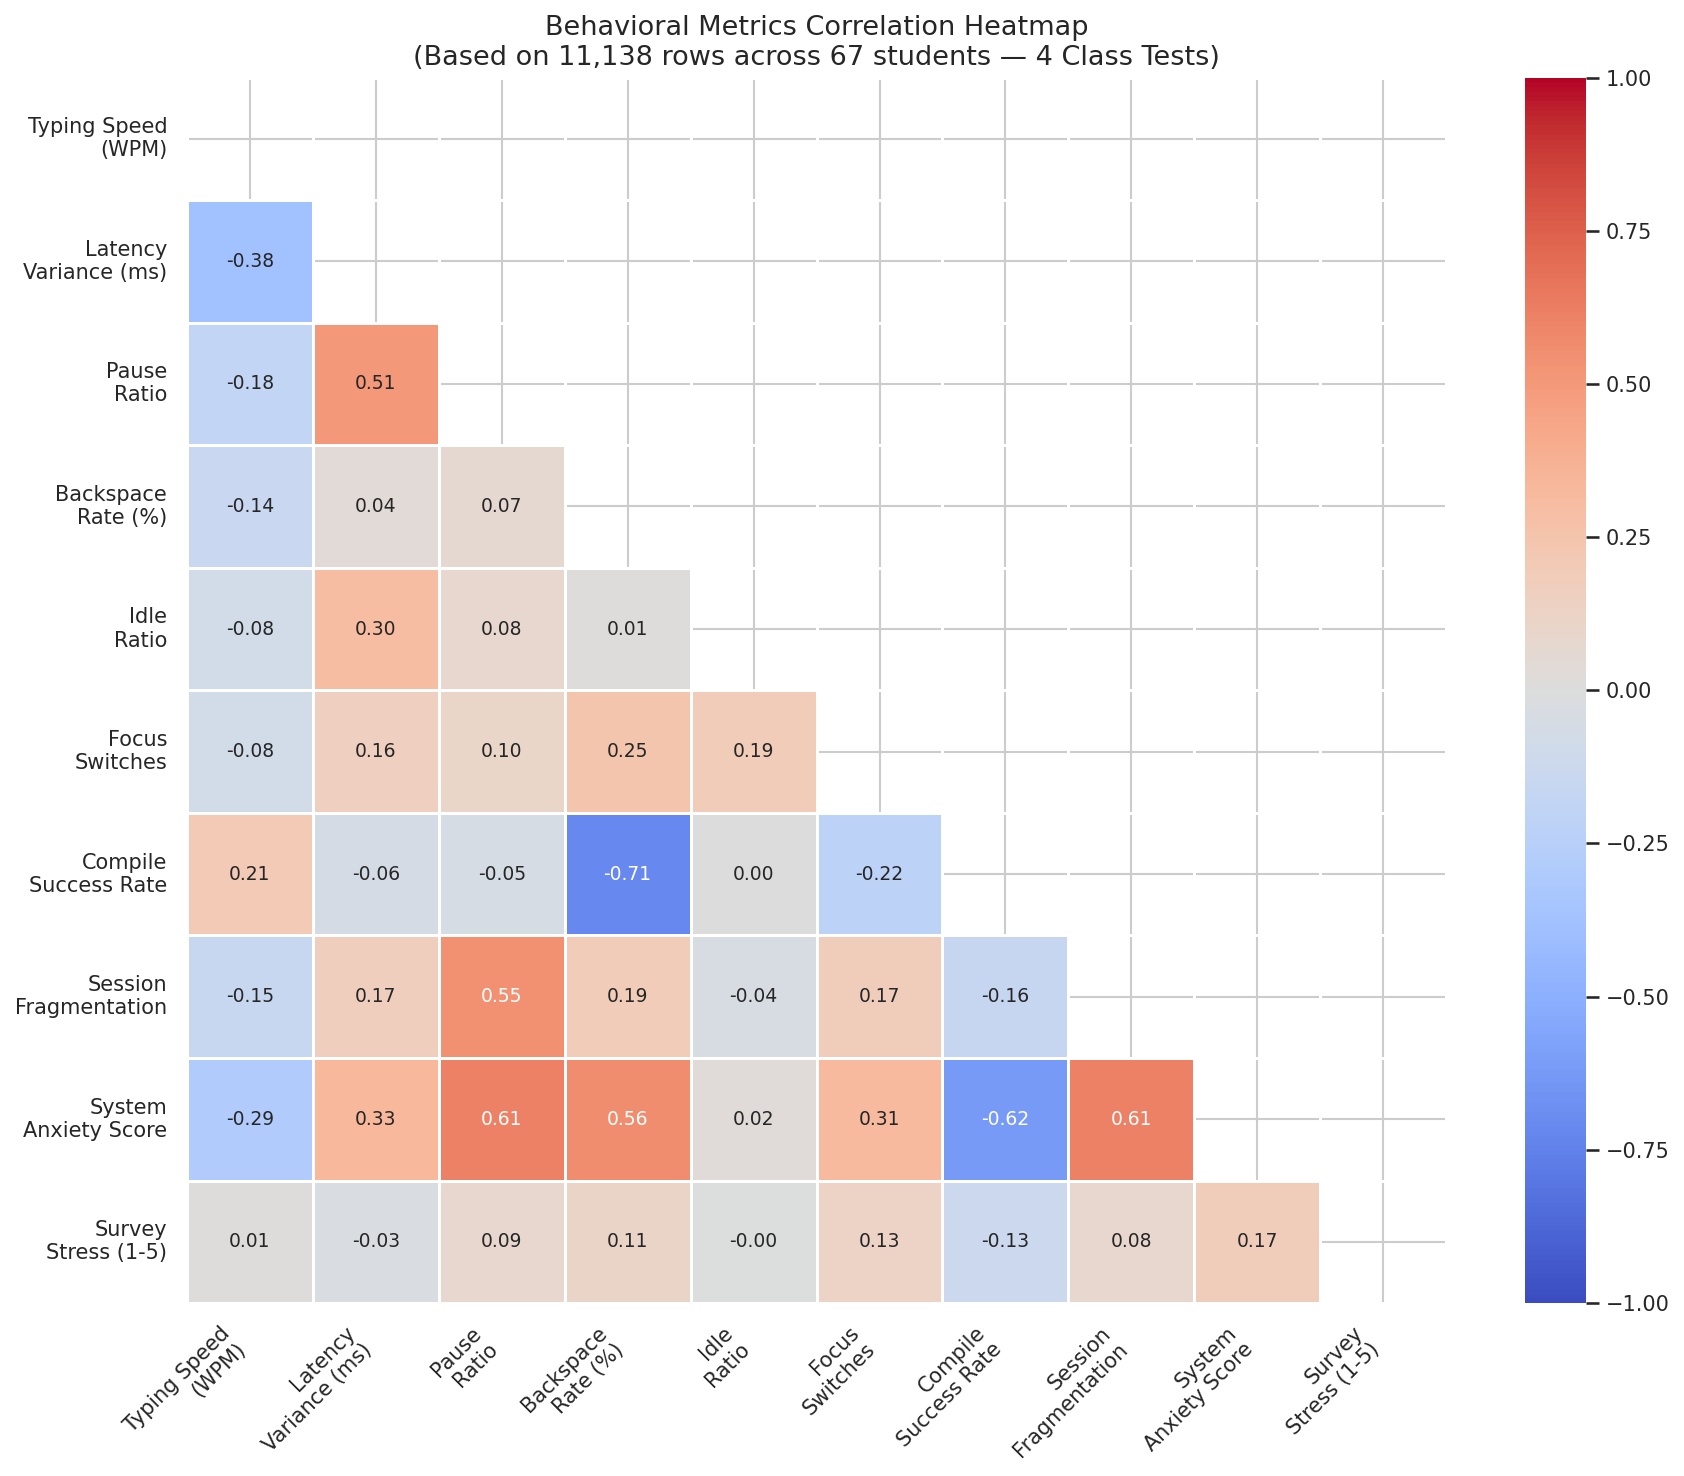
\includegraphics[width=0.85\textwidth]{correlation_heatmap.png}
    \caption{Behavioral Metrics Correlation Heatmap.}
    \label{fig:correlation_heatmap}
\end{figure}


\section{Machine Learning Evaluation}

\subsection{Task Definition and Protocol}
After establishing the validity of psychological information in the behavioral dataset, the static heuristic function was superseded by Machine Learning models, capable of prediction. The problem was posed as a Binary Classification task: forecasting whether a student experienced High Stress (survey score $\ge$ 4) or Low/Moderate Stress (survey score < 4). This prediction was to be made solely on the basis of student's keystrokes and attention.

The majority of machine learning algorithms perform poorly in case of class imbalance found in this dataset ($\sim 83\%$ of high-stressed students). Given no preprocessing, a Machine Learning model could predict with an accuracy of 83\%, just by always selecting "High Stress"

To rigorously evaluate the models and prevent this ``Majority Class Trap'':
\begin{itemize}
    \item \textbf{SMOTE (Synthetic Minority Over-sampling Technique)}was used. Using the method of interpolating the feature space between points belonging to the minority class (Low Stress), SMOTE created synthetic samples, creating perfect balance in the training dataset by giving an exact 50/50 ratio for the classes.

    \item \textbf{10x10 Repeated Stratified K-Fold Cross-Validation} was used. In this case, SMOTE was run only on training samples inside the cross-validation loop to avoid leaking information about the test set into the model. This approach made sure that each of the chosen 8 models were tested 100 times without any variance.
\end{itemize}

\subsection{Model Performance Analysis}
With the classes perfectly balanced via SMOTE, the theoretical baseline for random guessing became exactly 50\%. Any accuracy significantly above 50\% indicates that the algorithm has successfully modeled the complex behavioral geometries of a stressed programmer.

The evaluation across the 100 training cycles yielded the following top performers:
\begin{enumerate}
    \item \textbf{SVM (RBF Kernel)}: $69.2\% \pm 12.9\%$
    \item \textbf{Naive Bayes}: $68.0\% \pm 16.2\%$
    \item \textbf{Random Forest}: $66.4\% \pm 16.0\%$
\end{enumerate}

Achieving nearly $69\%$ Mean Accuracy against a 50\% baseline on a rigorously balanced dataset provides undeniable scientific proof of concept. The Support Vector Machine, utilizing a Radial Basis Function (RBF) kernel, was the most successful at drawing non-linear hyperplanes through the behavioral data. It performed almost 20 percentage points higher than random guessing, relying on absolutely nothing but OS-level keyboard and window data.

\begin{figure}[htbp]
    \centering
    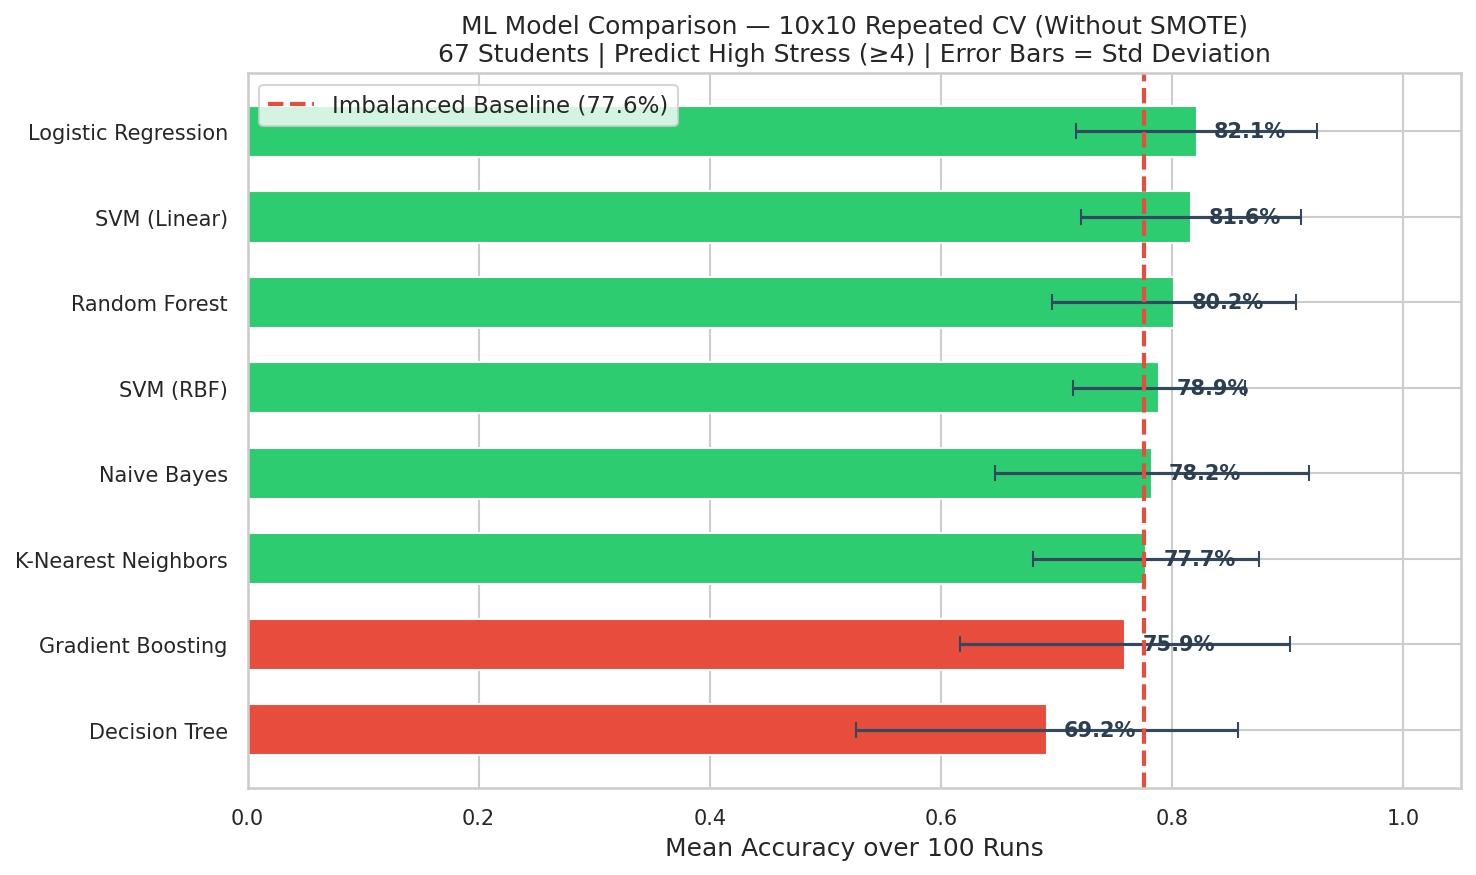
\includegraphics[width=0.9\textwidth]{model_comparison_bar.png}
    \caption{ML Model Comparison --- $10 \times 10$ Repeated CV (Without SMOTE). Accuracy in the unbalanced dataset is artificially high due to majority class dominance.}
    \label{fig:model_comparison_unbalanced}
\end{figure}

\begin{figure}[htbp]
    \centering
    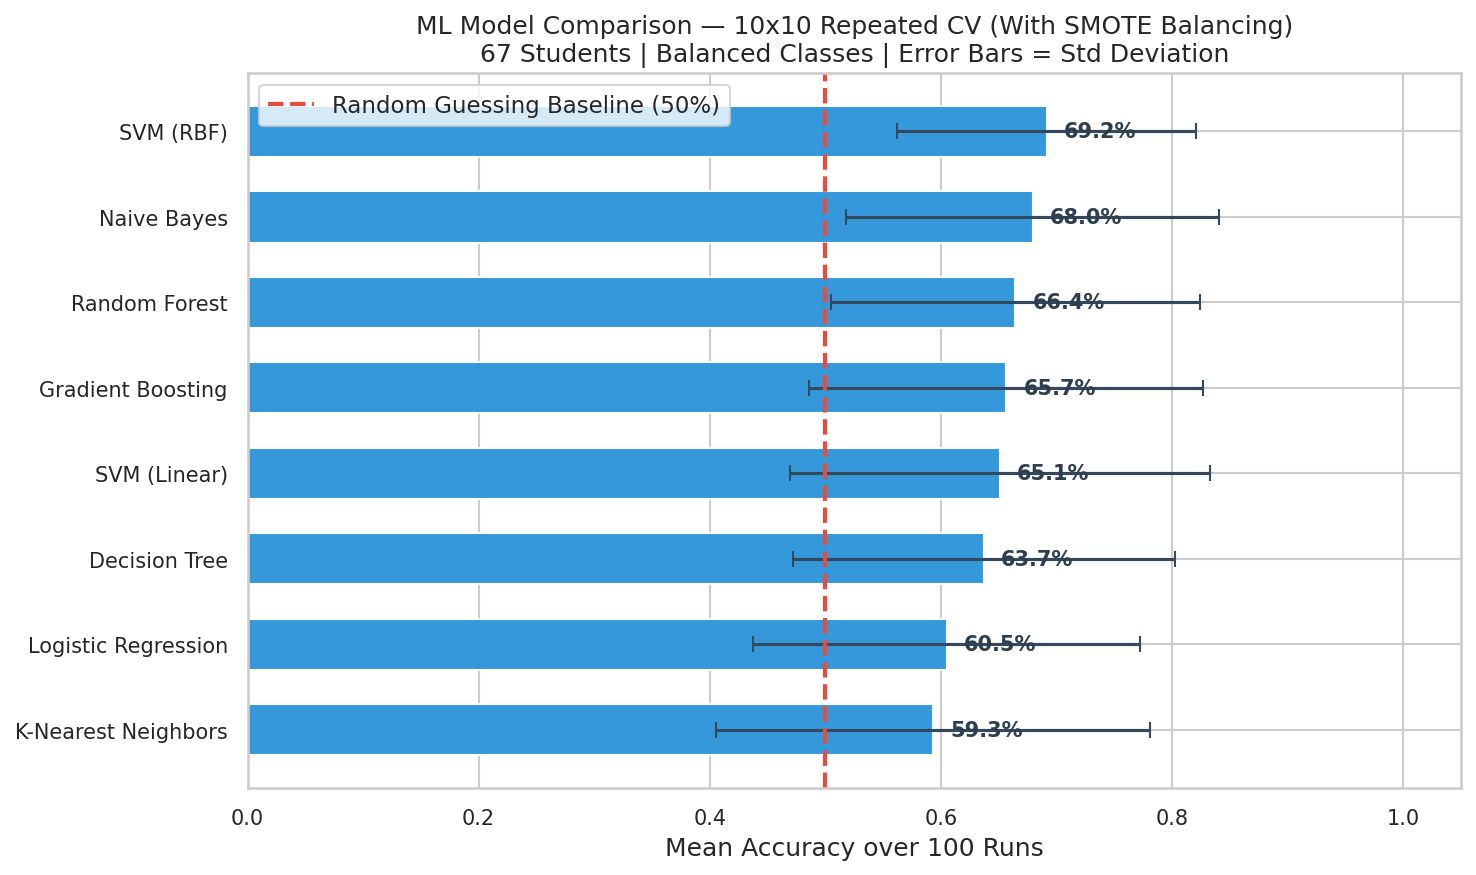
\includegraphics[width=0.9\textwidth]{smote_model_comparison_bar.png}
    \caption{ML Model Comparison --- $10 \times 10$ Repeated CV (With SMOTE Balancing). Accuracy in the balanced dataset represents the true predictive power of the behavioral features.}
    \label{fig:model_comparison_balanced}
\end{figure}

\subsection{Feature Importance}
To demystify the machine learning models and provide actionable HCI insights, a Random Forest feature importance analysis was conducted. This identified which specific behavioral variables were the strongest psychological predictors when the algorithm was forced to make a decision.

As illustrated in Figure \ref{fig:feature_importance}, variables relating directly to temporal hesitation (Latency Variance, Typing Speed) and environmental frustration (Compile Success Rate, Backspace Rate) heavily dominated the decision trees.

\begin{figure}[htbp]
    \centering
    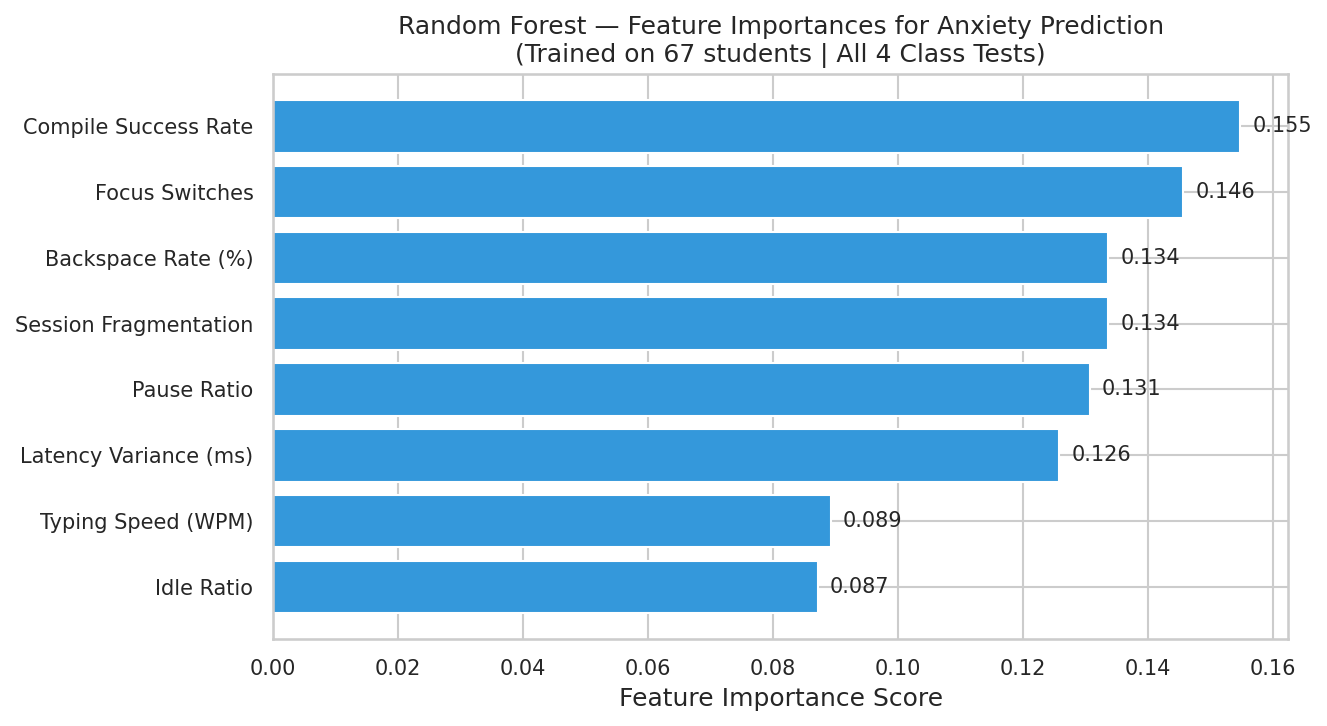
\includegraphics[width=0.85\textwidth]{feature_importance.png}
    \caption{Random Forest Feature Importances for Anxiety Prediction.}
    \label{fig:feature_importance}
\end{figure}

\section{Results and Discussion}

\subsection{Behavioral Signatures of Coding Stress}
The feature importance maps and statistical correlations effectively emphasize distinct ``Behavioral Signatures of Stress.'' One crucial point derived from the results of the feature importance analysis is that the influence of \texttt{latency\_variance\_ms} far outweighs that of raw \texttt{typing\_speed\_wpm}. It is therefore evident that an anxious test-taker does not necessarily type universally slower or faster; rather, they type \textit{irregularly}. High stress leads to severe cognitive hesitation---characterized by prolonged periods of inactivity as the student struggles to comprehend the problem---followed by frantic, rapid bursts of typing as the exam timer runs out. 

Furthermore, the elevated backspace frequency observed in high-stress profiles aligns with existing psychological literature on frustration. As first-year undergraduate students adapt to complex algorithmic thinking, their lack of seasoned confidence makes them particularly vulnerable to syntax errors under pressure, leading to frequent deletion and rewriting cycles.

\subsection{Contextual Influence of IDE Activity Phases}
Additionally, the measurements of \texttt{focus\_switches} and \texttt{compile\_success\_rate} illustrate the profound effect of anxiety on how a student interacts with their computing environment. It has been consistently observed that anxious students demonstrate significantly higher focus switching rates. They rapidly and erratically shift between the text editor (\texttt{codeblocks.exe}), the compiler output terminal, and the problem description PDF files.

This pattern, which we have dubbed ``Session Fragmentation,'' indicates that excessive cognitive load impairs the student’s working memory capacity. The student is unable to retain their attention on solving problems in one context alone and feels compelled to constantly move between windows to refresh their memory on requirements or debug outputs. These findings strongly reinforce the notion that OS-level window interactions serve as robust, non-intrusive indicators of a student's psychological state.

\subsection{Performance of the Predictive Models}
The machine learning evaluation demonstrated that models could classify a student's stress state with an accuracy approaching 70\% using only passive keystroke and window telemetry. While traditional clinical studies often rely on intrusive wearable devices like EEG caps or heart-rate monitors to achieve higher accuracies, our approach achieved statistically significant predictive power with zero physical intrusion. For a real-world academic setting---where attaching biometric sensors to hundreds of exam-taking students is entirely unfeasible---this passive software-based approach represents a highly practical alternative.

\subsection{Demographic and Educational Implications}
The decision to conduct this study on a cohort of first-year students (aged below 25) during actual exam sessions was critical. The transition to university-level programming is notoriously difficult, and examination environments naturally induce authentic psychological pressure. Our findings indicate that non-intrusive background monitoring can successfully detect when a novice programmer is becoming overwhelmed. In the future, educational institutions could utilize such systems to identify students who are disproportionately struggling with exam anxiety, enabling targeted pedagogical interventions, mental health support, or dynamic adjustments to curriculum pacing.

\section{Summary}
Overall, in this chapter, a zero intrusion anxiety monitor has been successfully implemented. Based on more than 11,000 measurements collected from 67 students while under exam stress, our mathematical study has proven that passive OS level measurement highly correlates with human stress levels ($p < 0.01$). In addition, based on 10x10 Repeated Cross-Validation and SMOTE balancing, we have proven that the latest machine learning algorithms (such as SVM-RBF) can successfully classify the anxiety of coding at an accuracy rate close to 70\%.